\documentclass[12pt]{article}
\usepackage[utf8]{inputenc}
\usepackage[english]{babel}
\usepackage{amssymb}
\usepackage{stmaryrd}
\usepackage{enumitem}
\usepackage{amsmath}
\usepackage{array}
\usepackage[left=2cm,right=2cm,top=2cm,bottom=2cm]{geometry}
\usepackage[T1]{fontenc}
\setlength\parindent{0pt}
\usepackage{graphicx}
\usepackage[ddmmyyyy]{datetime}

\usepackage[backend=biber]{biblatex}
\addbibresource{ref.bib}

\usepackage{booktabs}
\usepackage{float}
\usepackage{forest}
\usepackage{setspace}
\usepackage{hyperref}
\hypersetup{
    colorlinks=true,
    linkcolor=blue,
    filecolor=magenta,      
    urlcolor=cyan,
}
\usepackage{easytable}
\usepackage{adjustbox}
\usepackage{listings}
\lstdefinelanguage{Matlab}%
  {morekeywords={matlab2tikz},
   morekeywords=[2]{1}, 
   morekeywords=[3]{xlim,ylim,clim,iter},
   morekeywords=[4]{x,y,scatter,contour,imagesc,addplot3},
   morecomment=[l][\color{blue}]{...},%
   morestring=[m]',%
   morestring=[m]"%
  }[keywords,comments,strings]

\lstset{%
  language=Matlab,%
  breaklines=true,%
  morekeywords={matlab2tikz},
  keywordstyle=\color{blue},%
  morekeywords=[2]{1}, keywordstyle=[2]{\color{black}},
  identifierstyle=\color{black},%
  stringstyle=\color{mylilas},
  commentstyle=\color{mygreen},%
  showstringspaces=false,
  numbers=left,%
  numberstyle={\tiny \color{black}},
  numbersep=9pt,
  emph=[1]{for,end,break},emphstyle=[1]\color{red},
}

\hypersetup{
    colorlinks=true,
    linkcolor=black,  % Changer la couleur ici
    filecolor=magenta,      
    urlcolor=cyan,
}

\usepackage{tikz}
\usetikzlibrary{calc}

\renewcommand{\dateseparator}{/}

\usepackage{fancyhdr}
\usepackage{lastpage}

\pagestyle{fancy}
\renewcommand\headrulewidth{1pt}
\renewcommand\footrulewidth{1pt}
\geometry{headsep=1.1cm}

\newtheorem{theorem}{Théorème}[subsection]
\newtheorem{corollary}{Corollaire}[theorem]
\newtheorem{lemma}[theorem]{Lemme}
\newtheorem{definition}{Définition}[subsection]
\newtheorem{proposition}{Proposition}[section]

\fancyhead[L]{
\includegraphics[width=0.1\columnwidth]{./logo}~}
\fancyfoot[L]{\textsc{Machine Learning
}}
\fancyhead[R]{\textsc{Edward LUCYSZYN}}
\fancyfoot[C]{\thepage/\pageref{LastPage}}
\fancyfoot[R]{\textsc{\today}}

\usepackage{xcolor}
\usepackage{piton}
\usepackage{tcolorbox}
\newcommand{\Tr}{\operatorname{Tr}}
\newcommand{\Arg}{\operatorname{Arg}}

\usepackage{amsmath}
\DeclareMathOperator*{\argmax}{argmax}
\DeclareMathOperator*{\argmin}{argmin}

%====================== INFORMATION ET REGLES ======================

%rajouter les numérotation pour les \paragraphe et \subparagraphe

\setcounter{tocdepth}{4}
\setcounter{secnumdepth}{0}


%======================== DEBUT DU DOCUMENT ========================

\begin{document}

% \NewPitonEnvironment{Python}{O{}}{\PitonOptions{#1}}{}
\PitonOptions{break-lines, indent-broken-lines}

\NewPitonEnvironment{Python}{}
  {\begin{tcolorbox}[breakable]}
  {\end{tcolorbox}}


%régler l'espacement entre les lignes
\newcommand{\HRule}{\rule{\linewidth}{0.5mm}}

%page de garde
\begin{titlepage}
\begin{center}

% Upper part of the page. The '~' is needed because only works if a paragraph has started.

\LARGE \textsc{2EL1740: Algèbre \& Cryptologie}

\vspace{0.2cm}

\Large \textsc{CentraleSupélec - 2A}

\vspace{0.3cm}

% Title
\HRule \\[0.4cm]

{\huge \bfseries Challenge 4\\
[0.2cm]}

\HRule \\[0.4cm]

\vspace{2cm}

\textsc{\today}

\vspace{2cm}


\includegraphics[width=0.4\columnwidth]{./logo}~\\[3cm]

% Author and supervisor
\begin{minipage}{0.4\textwidth}
\begin{spacing}{1.125}
\begin{center}
    Raphaël \testsc{PAIN DIT HERMIER}\\
    Alexis \testsc{LOMBARD-GAILLARD}\\
    Edward \testsc{LUCYSZYN}
\end{center}
\end{spacing}
\end{minipage}

\vfill

\end{center}
\end{titlepage}

%page blanche
%\newpage
%~
%ne pas numéroter cette page
\thispagestyle{empty}

\tableofcontents
\thispagestyle{empty}
% \setcounter{page}{1}
%ne pas numéroter le sommaire

%\newpage

%espacement entre les lignes d'un tableau
\renewcommand{\arraystretch}{1.5}

%====================== INCLUSION DES PARTIES ======================

~
\thispagestyle{empty}
%recommencer la numérotation des pages à "1"
\setcounter{page}{0}

\newpage

\section{One-Dimensional Schrödinger Equation}

\noindent The goal is to establish the necessary mathematical foundations to better understand and assimilate the concepts of wave function and the resolution of the Schrödinger equation.

\subsection{First Order Equations}
\noindent Consider the following time-dependent equation:
\begin{equation}
    \forall t \in \mathbb{R}_{+}, \quad \frac{df}{dt}(t) = af(t)
\end{equation}
where $\displaystyle a=-\frac{1}{\tau}$ is a real constant ($\tau >0$).\\ \\

\noindent \textbf{1)} Find the set of solutions to the differential equation. What is the dimension of $\tau$?\\

\begin{breakbox}
\noindent This is a first-order differential equation. We know that $f$ has the form: $$\boxed{\forall t \in \mathbb{R}_{+}, \quad f(t)=Ae^{at}}$$ 
where $A$ is a constant (in $\mathbb{C}$ generally) that depends on an initial condition (or normalization condition). $\tau$ has the dimension of time. It is often referred to as the \textbf{characteristic time}.
\end{breakbox}

\subsection{Second Order Equations}

\begin{equation}
    \frac{d^2\phi}{dx^2}(x) = b\phi(x)
    \label{equ2}
\end{equation}

\noindent
where $b$ is a nonzero real constant.\\ \\

\noindent \textbf{2)} Find the set of solutions to the differential equation. Solutions can be sought in exponential form, distinguishing different cases based on the sign of $b$.\\

\begin{breakbox}

\noindent There are several methods to solve this second-order differential equation.\\ \\
\noindent \textbf{Method 1: Seeking solutions of the form $\phi (x) = Ae^{cx}, c \in \mathbb{R}$.}\\
We seek solutions in exponential form (this point is admitted). So, $$\phi (x) = Ae^{cx}$$ with $c$ to be determined.
We substitute this solution into the differential equation (2): $$c^2Ae^{cx} = b Ae^{cx}.$$
By simplifying with $\phi (x)= Ae^{cx}$ ($A \neq 0$), we obtain: $c^2 = b$. \\ \\Here we distinguish two cases:

\begin{itemize}
    \item If $b<0$: we set $b=(ik)^2$, with $k > 0$. Then we have the equality $c^2 = (ik)^2$, 
resulting in $c = \pm ik$. There are thus two forms of exponential solutions, one in $ikx$ and the other in $-ikx$. Since these two solutions are independent, the general solution for $\phi$ is: $$\boxed{\phi(x) = Ae^{ikx} + Be^{-ikx}.}$$
    \item If $b>0$: we set $b=k^2$. Then we find $c = \pm k$.
As before, we find two forms of independent exponential solutions, and the general solution is: $$\boxed{\phi = Ae^{kx} + Be^{-kx}.}$$
\end{itemize}
\textbf{Method 2: Passing through the characteristic equation.}\\
We write the characteristic equation (or polynomial) in $X$ associated with the differential equation (2), which is:
\begin{equation}
    X^2 - b = 0.
    \label{eq3}
\end{equation}
We also know that the solutions to (\ref{equ2}) are of the form $\psi(x) = Ae^{r_1x}+Be^{r_2x}$ where $r_1, r_2 \in \mathbb{C}$ are the complex roots of equation (\ref{eq3}).\\
We then distinguish the cases $b >0$ and $b<0$ as detailed in Method 1.

\end{breakbox}

\subsection{Variable Separation and Schrödinger}

\noindent Let $\psi$ be a function of two variables that satisfies the one-dimensional Schrödinger equation: 
\begin{equation}
    \forall (x, t) \in \mathbb{R} \times \mathbb{R}_{+}, - \frac{\hbar ^2}{2m}\frac{\partial^2\psi(x,t)}{\partial x^2} = i\hbar\frac{\partial\psi(x,t)}{\partial t}.
\end{equation}
\noindent Furthermore, suppose that $\psi$ can be written in the form: 
\begin{equation}
    \psi(x,t) = \phi(x)f(t).
\end{equation}


\noindent \textbf{3.a)} Simplify the equation to obtain a term dependent only on $x$ and another term dependent only on $t$. What can be concluded from this equality? \\

\begin{breakbox}
\noindent We first notice that $$\frac{\partial^2\psi(x,t)}{\partial x^2} = \frac{\partial^2\phi(x)f(t)}{\partial x^2} = f(t)\phi^{''}(x).$$
Likewise:  $$\frac{\partial\psi(x,t)}{\partial t} = \phi(x)\dot{f}(t).$$
Knowing this, we rewrite the Schrödinger equation: $$- \frac{\hbar ^2}{2m}f(t)\phi^{''}(x) = i\hbar\phi(x)\dot{f}(t).$$
Thus finally:
$$\boxed{-\frac{\hbar ^2}{2m}\frac{\phi^{''}(x)}{\phi(x)} = i\hbar\frac{\dot{f}(t)}{f(t)}.}$$\\

\noindent We obtain an equality between an expression dependent only on $x$ and another dependent only on $t$.
Therefore, we conclude that the equality must necessarily be equal to a constant, which we denote $E \in \mathbb{R}$.
\end{breakbox} 

\medskip

\noindent \textbf{3.b)} Deduce the differential equations satisfied by $\phi$ and $f$. Provide the dimension and physical meaning of the introduced constant.\\

\begin{breakbox}

\noindent The constant $E$ has dimensions of energy, which can be seen by examining the dimension of one of the two terms. For example: 
$$[E]=[\frac{\hbar ^2}{2m}\frac{\phi^{''}(x)}{\phi(x)}\big] = [\frac{\hbar ^2}{2m}] L^{-2} = [\frac{\hbar^2 k^2}{2m}] = [\frac{p^2}{2m}] = Energy$$ \\ \\
We then obtain the following two differential equations:

\begin{equation}
    \boxed{\dot{f}(t) = \frac{E}{i\hbar}f(t);}
    \label{a1}
\end{equation}

\begin{equation}
    \boxed{\phi^{''}(x) = -\frac{2mE}{\hbar^2}\phi(x).}
    \label{a2}
\end{equation}
\end{breakbox}

\medskip

\noindent \textbf{3.c)} Then give the general form of the solutions for $\psi(x,t)$ depending on the sign of the introduced constant.\\

\begin{breakbox}
\noindent Here it is a matter of recognizing the forms of the differential equations from questions 1.1 for equation (\ref{a1}), and 1.2 for equation (\ref{a2}). Thus $$f(t)= Ae^{-i \frac{Et}{\hbar}}.$$\\ \\

\begin{itemize}
    \item If $E$ is negative, (\ref{a2}) becomes $$\phi^{''}(x) = \frac{2m|E|}{\hbar^2}\phi(x)$$ and according to 1.2:
    $$\phi(x) = Ae^{kx} + Be^{-kx}\text{, where } k^2 = -\frac{2mE}{\hbar^2}.$$ Finally:
    $$\boxed{\psi(x,t) = (Ae^{kx} + Be^{-kx})e^{\frac{-iEt}{\hbar}}.}$$
    \\
    \item Conversely, if $E$ is positive, then as shown in question 2, the solution will be of the form $\phi(x) = Ae^{ikx} + Be^{-ikx}$, with $\displaystyle k^2 = \frac{2m
    E}{\hbar^2}.$ \\ \\        Finally: $$\boxed{\psi(x,t) = (Ae^{ikx} + Be^{-ikx})e^{\frac{-iEt}{\hbar}}.}$$
\end{itemize}
\end{breakbox}


\newpage
\section{Model tuning and comparison}

After studying and formatting the data, we tested different models for this problem, starting with a basic model and then moving on to more complex approaches.

\subsection{k-Nearest Neighboors}

The simplest algorithm is arguably the k-Nearest Neighbors (kNN). It was the example algorithm for the project. It achieved an accuracy of 33\% on the test data. We used it very little because we immediately had many features, and with a high number of dimensions, the concept of distance becomes redundant.

\subsection{SVM}

Another algorithm we tried was the Support Vector Machine (SVM). We used a Gaussian kernel for which we found the theta by performing cross-validation with the \texttt{GridSearch} function. However, we did not initially achieve good results, even worse than those of the k-NN. This can be explained either by the fact that the model was not suitable for the problem, or that our training data formatting was not as good at the time, which skewed the results.

\subsection{Random Forests}

One of the more complex models we tested was Random Forest. To do this, we used the \texttt{RandomForest} and \texttt{GridSearch} functions from \texttt{ScikitLearn}. This model is well-suited to our problem because it does not necessarily require normalizing the data, which is perfect since we have continuous and discrete numerical information. Additionally, it is easy to parallelize with Random Forests, which significantly reduces computation time. After reformatting the initial data, we achieved a maximum score of approximately 0.97.

\subsection{Chosen solution}

We therefore chose the model with Random Forest. We also attempted to build a neural network, but the code was complicated to understand and did not yield good results, leading us to believe that we made a mistake. Since Random Forest already provided satisfactory results, we did not delve further into the issue.

\begin{center}
\begin{tabular}{|c|c|}
\hline
Model & Score \\
\hline
kNN &  Between 0,30 and 0,40 \\
SVM & Less than 0,20 \\
RandomForest & Around 0,97 \\
\hline
\end{tabular}
\end{center}

\newpage
\section{Orders of Magnitude}

\noindent \textbf{1)} Consider a monoatomic gas, ${ }^4 \mathrm{He}$ for example, at room temperature. The particles are free, and it will be shown later in this course that the average kinetic energy per atom is $\displaystyle \frac{3}{2} k_B T$. What is the de Broglie wavelength $\lambda_{dB}$ associated with each of these gas atoms?\\

\begin{breakbox}
    \noindent Let's first calculate the characteristic energy corresponding to room temperature. This value will be often used later in the course. The quantity $k_BT$ at 300 K is $4.14 \times 10^{-21}$ J, or $2.6 \times 10^{-2}$ eV. So approximately $k_BT \approx 1/40$ eV at room temperature.\\ \\
    \noindent Therefore, we have:
    $$\boxed{E_{He} = \frac{\hbar^2(2\pi)^2}{2m_{He}}{\lambda_{dB}^2}.}$$  
    \noindent and $m_{He} = \frac{4 \times 10^{-3}}{6.02 \times 10^{23}} = 0.66 \times 10^{-26}$ kg. We find $\lambda_{dB} = 7.45 \times 10^{-11}$ m = 0.745 Angströms.
\end{breakbox}

\medskip

\noindent \textbf{2)} Knowing that the density of the gas is approximately $n=10^{24}$ atoms/$\mathrm{m}^3$ (pressure close to atmospheric), compare the obtained wavelength to the average distance between atoms, $\bar{d}$.\\

\begin{breakbox}
    \noindent In order to compare this result to a characteristic length of the system, let's estimate the average distance between the gas atoms. The density is $n = 10^{24}\ \mathrm{m}^{-3}$; we deduce an average distance of about $\displaystyle \boxed{\bar{d} \approx n^{-1/3} \approx 10^{-8}\ \mathrm{m}.}$ So $\lambda_{dB} \ll \bar{d}$.
\end{breakbox}

\medskip

\noindent \textbf{3)} What happens if the temperature is lowered to $10^{-6} \mathrm{~K}$ as allowed by laser cooling technique (Nobel 1997)? Show that the condition $\lambda_{dB} \ll \bar{d}$ is an essential condition for classical physics to still be applicable.\\

\begin{breakbox}
    \noindent The fact that $\lambda_{dB} \ll \bar{d}$ means that on average, it will be very difficult to observe any interference effects between the waves associated with the gas atoms.\\ \\
    Consequently, one can expect quantum effects to be negligible. There are several criteria to decide whether quantum physics is appropriate (and necessary) for describing a particular system (see course).\\ \\
    However, if the helium atom's wavelength is so small, it's because the mass is greater than that of a simple electron, but also because the thermal energy is not negligible.\\
    Therefore, let's consider what happens if we are able to considerably cool down this gas, thus slowing it down. The available energy is now about $10^{-8}$ times lower.
    Since the square of the wavelength varies inversely with energy, it will be itself $10^4$ times larger and of the order of $10^{-7}\ \mathrm{m}$.
    It is then no longer negligible compared to the average distance between atoms in the gas: interference phenomena can then become observable.
    At these very low temperatures, quantum physics becomes indispensable because its effects dictate the behavior of the system.
\end{breakbox}

\section{Photoelectric Effect}

\noindent Zinc is one of the metals used in the experiment by Von Lenard to demonstrate the photoelectric effect. The work function of an electron from zinc, i.e., the energy required to release this electron from the attractive potential of the metal ions, is about $4.3 \mathrm{eV}$. By illuminating the zinc with radiation of wavelength $\lambda \approx 200 \mathrm{~nm}$ (far UV) and power $1 \mathrm{~mW}$, what is the maximum power carried by the electron beam?\\

\begin{breakbox}
    \noindent At a wavelength of $\lambda \approx 200$ nm, the energy of each photon is about $$E = \frac{hc}{\lambda} = \frac{(6.626 \times 10^{-34}) \times (3.00 \times 10^8)}{200 \times 10^{-9}} \approx 9.94 \times 10^{-19} \, \mathrm{J} \approx 6.21\ \mathrm{eV}.$$
    For a power of $P = 1\ \mathrm{mW}$, there are then $$n = \frac{P}{E} \approx \frac{10^{-3}}{6,2\times 1,6 \times 10^{-19}} \approx 10^{15}\ \mathrm{photons/s}$$ incident on the surface of the metal.\\ \\
    Assuming that each photon is absorbed by a zinc atom and serves to eject an electron, we can expect that there are also about $10^{15}$ electrons emitted per second.
    However, the electrons will each have a much lower energy since 4.3 eV has been spent each time to release the electron.
    Therefore, each electron can only leave with $6.21 - 4.3 = 1.89\ \mathrm{eV}$ of kinetic energy.\\ \\
    Thus, the electron beam will have at most a power of: $$\boxed{P_f = 1.89 \times 1.6 \times 10^{-19}\times 10^{15} \approx 0.302\ \mathrm{mW}.}$$
\end{breakbox}

\newpage
\section{Blackbody Radiation and Wien's Displacement Law}

\noindent \textbf{1)} At the limit of small wavelengths, show that the Planck distribution has a maximum at the wavelength $\lambda_{\max}$ such that $\lambda_{\max} T=C$, where the value of $C$ depends on Planck's constant $h$.\\

\begin{breakbox}
    \noindent At the limit of small wavelengths, the Planck distribution (or Planck's law) is given by:
    $$dU \approx \frac{8\pi h c}{\lambda^5}e^{-hc/(\lambda k_B T)}d\lambda.$$
    Thus, we obtain $\displaystyle \frac{dU}{d\lambda} \approx 0$ when:
    $$\boxed{\lambda_{max} T \approx \frac{hc}{5k_B}.}$$
\end{breakbox}

\medskip

\noindent \textbf{2)} Use the experimental value $C=2.9 \mathrm{~mm} . \mathrm{K}$ to deduce an approximate value of $h$.\\

\begin{breakbox}
    \noindent The product of $\lambda_{max}$ and $T$ is indeed a constant $C$ which is $C = h \times 0.434 \times 10^{31}$ m.K.
    This result can be compared to the experimental value $C \approx 2.9 \times 10^{-3}$ m.K to find an approximate value of $h \approx 6.68 \times 10^{-34}$ J.s.
\end{breakbox}


\newpage


\section{Kapitza-Dirac Prediction}

\noindent In 1933, Kapitza and Dirac proposed that the diffraction of an electron beam by a lattice formed of stationary electromagnetic waves could be observed. Because this relies on the process of stimulated emission, they predicted that the probability of such a process would be very low and would require a very intense light source to enhance the electron-photon interaction. Indeed, this technical feat had to wait 70 years for the advent of very powerful lasers. Figure~\ref{fig:Kapitza-Dirac} summarizes the principle of the experiment and its results.

\begin{figure}[H]
    \centering
    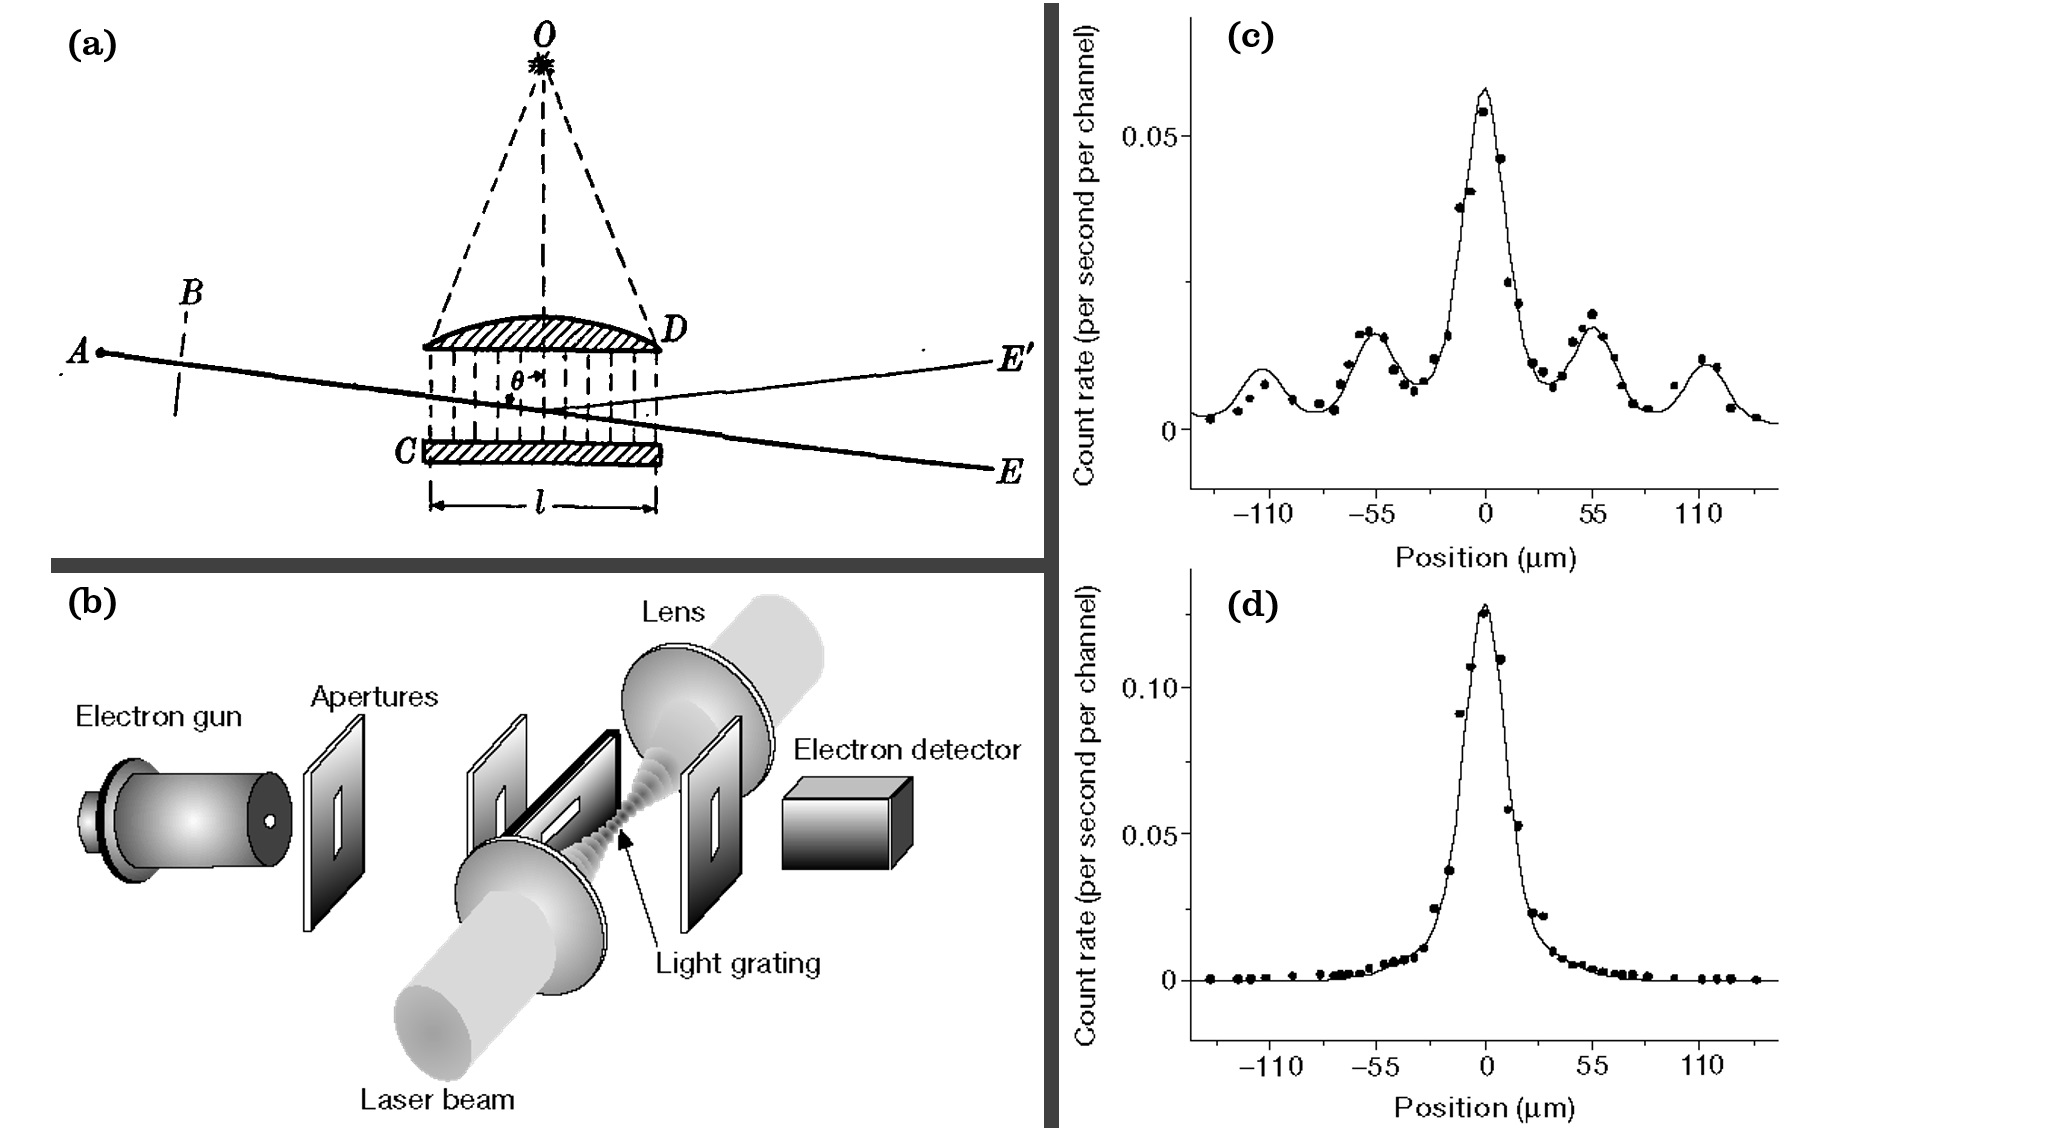
\includegraphics[width=\textwidth]{Kapitza-Dirac.jpg}
    \caption{Diffraction of massive particles by stationary electromagnetic waves. (a) Principle as described in Kapitza and Dirac's publication (1933). Electrons are emitted at $A$ and detected at $E^{\prime}$ when the lattice is created between lens $D$ and mirror $C$. When the light is off, the particles should be detected at $E$. (b) Experimental setup by Freimund and colleagues. (c) Interference fringes as seen by the detector at a distance of $24 \mathrm{~cm}$ from the lattice. The abscissa refers to the detector position. (d) Detected signal when the electromagnetic wave is turned off. Adapted from Nature, "Observation of the Kapitza-Dirac effect", Freimund, Kayvan, Aflatooni and Batelaan, \copyright \,2001.}
    \label{fig:Kapitza-Dirac}
\end{figure}

\noindent \textbf{1)} The electrons have an energy of about $380$ eV. What is the wavelength $\lambda_e$ of the incident electron beam?\\

\begin{breakbox}
    \noindent The wavelength is $\boxed{\lambda_e = \frac{2\pi}{k} = \frac{2\pi}{\sqrt{2m\epsilon_e}}\approx 0.6\ \text{Angstroms}.}$
\end{breakbox}

\medskip

\noindent \textbf{2)} The laser beam has a wavelength $\lambda_\nu=532$ nm. What is the energy of the photons? To achieve high power, the laser must operate with $10$ ns pulses, each carrying $0.2$ J. What is the photon flux (in $\mathrm{W/m^2 s}$) if the beam has a diameter of $125\ \mu \mathrm{m}$?\\

\begin{breakbox}
    \noindent Firstly, the energy of the photon is $\displaystyle \epsilon_{\nu} = \frac{2\pi\hbar c}{\lambda_{\nu}}\approx 3.7 \times 10^{-19}$ J $\approx 2.3$ eV. Secondly, the surface power density of the LASER is $\displaystyle d^{surf}_{P}=\frac{E_{pulse}}{\sigma \times \Delta t}$ with $\sigma$ the cross-section of the LASER beam, $\Delta t$ the time gap between each pulse, and $E_{pulse}$ the energy delivered by the LASER during a pulse. Thus, $\displaystyle d^{surf}_{P}=\frac{0.2}{10 \times 10^{-9}\times \pi \times (62.5 \times 10^{-6})^2} \approx 1.6 \times 10^{15} \: \mathrm{W/m^2}$. Finally, the photon flux is $\displaystyle \frac{d^{surf}_{P}}{\epsilon_{\nu}} = \frac{1.6 \times 10^{15}}{3.7 \times 10^{-19}} \approx 4.4 \times 10^{33} \: \mathrm{photons / (m^2 s)}$.
\end{breakbox}

\medskip

\noindent \textbf{3)} Justify the presence of a first-order diffraction peak at $55 \mu \mathrm{m}$ using the diffraction law $d \sin \theta=n \lambda$, where $d$ is the lattice period, $\lambda$ is the wavelength of the incident radiation, and $\theta$ is the diffraction angle.\\

\begin{breakbox}
    \noindent The light gridding (i.e., two-dimensional lattice) is created by the intensity of the diffracted radiation. Thus, the period is half a wavelength $\displaystyle d = \frac{\lambda_{\nu}}{2} = 532/2$ nm. Using the diffraction law for the first order ($n = 1$), we find that the angle corresponding to the first diffraction peak is $\displaystyle \theta_1 = \frac{2 \times 0.6 \times 10^{-10}}{532 \times 10^{-9}} \approx 0.226 \times 10^{-3}$ rad, and the detector for this first maximum is placed at $x_1 = 0.226 \times 10^{-3} \times 0.24 \approx 54 \mathrm{\mu m}$.
\end{breakbox}


\newpage
\section{Wave Functions, Energies, and Observables}

\noindent For the rest of the tutorial, we will try to visualize wave functions and their associated energies in the case of the infinite well, recalling and developing points that have been addressed in class. \\ \\
Go to: \url{http://prd-mecaqu.centralesupelec.fr/FR/ex1.html}.\\ \\
\underline{Instruction}: Uncheck the "Afficher la probabilité" box. \\ \\
We provide again the wave functions and energies of a particle in an infinite potential well, as you established in Tutorial 2 of Physics:

\begin{equation}
    \phi_n(x) = \sqrt{\frac{2}{a}}\sin(\sqrt{\frac{2mE_n}{\hbar^2}}x)~~ \text{and} ~~ E_n = \frac{\hbar^2n^2\pi^2}{2ma^2}.
\end{equation}

\subsection{Wave Function and Probability Density}

\noindent \textbf{1.a)} Express, in terms of $\phi_n$, the probability of finding the particle on the interval $[x, x + dx]$.\\

\begin{breakbox}
    \noindent By definition of the probability density:
    $$\boxed{\text{d}P = \vert \phi_n(x) \vert^2 \text{d}x.}$$
\end{breakbox}

\medskip

\noindent \textbf{1.b)} Give the probability of finding the particle outside the infinite well $P_1$, and the probability of finding it within the well $P_2$, i.e., between $[0, a]$. We recall that $\displaystyle \int_{0}^{b} \sin^{2}(x) \mathrm{d}x = \frac{b}{2} - \frac{\sin(2b)}{4}.\\

\begin{breakbox}
    \noindent We have, outside of $[0, a]$:
    $$
    \boxed{P_1 = \int_{\mathbb{R} \setminus [0,a]} |\phi_n(x)|^2 \, \mathrm{d}x = 0}
    $$
    because $\vert \phi_n(x) \vert^2 = 0.$\\ \\
    Then,
    \begin{align*}
    P_2 &= \int_{0}^{a} |\phi_n(x)|^2 \, \mathrm{d}x \\
    &= \int_{0}^{a} \frac{2}{a}\sin^2\left(\sqrt{\frac{2mE_n}{\hbar^2}}x\right) \mathrm{d}x \\
    &= \int_{0}^{a} \frac{2}{a}\sin^2\left(\frac{n\pi}{a}x\right) \mathrm{d}x \\
    &= \frac{2}{n\pi} \int_{0}^{n\pi} \sin^2(y) \mathrm{d}y \\
    &= \frac{2}{n\pi}\left(\frac{n\pi}{2} - \frac{\sin(2n\pi)}{4}\right).
\end{align*}
\noindent So
    \[
        \boxed{P_2 = 1.}
    \]
\noindent This is a result that we could have expected since the particle remains confined in the well; we cannot find it outside. Thus, it only exists within $[0, a]$, and therefore $P_2 = 1$.
\end{breakbox}

\subsection{Boundary Conditions}

\noindent \textbf{2.a)} Given the probability density conditions found above, give the boundary conditions of the well for the wave function $\phi_n$. \\

\begin{breakbox}
    \noindent As seen in class, we have:
    \[
    \boxed{\phi_n(0) = 0 \text{ and } \phi_n(a) = 0.}
    \]
\end{breakbox}

\medskip

\noindent \textbf{2.b)} On the website, go to the "Wave function" section. What do you notice about the derivative of $\phi_n$ at the boundaries of the well? \\

\begin{figure}[H]
    \centering
    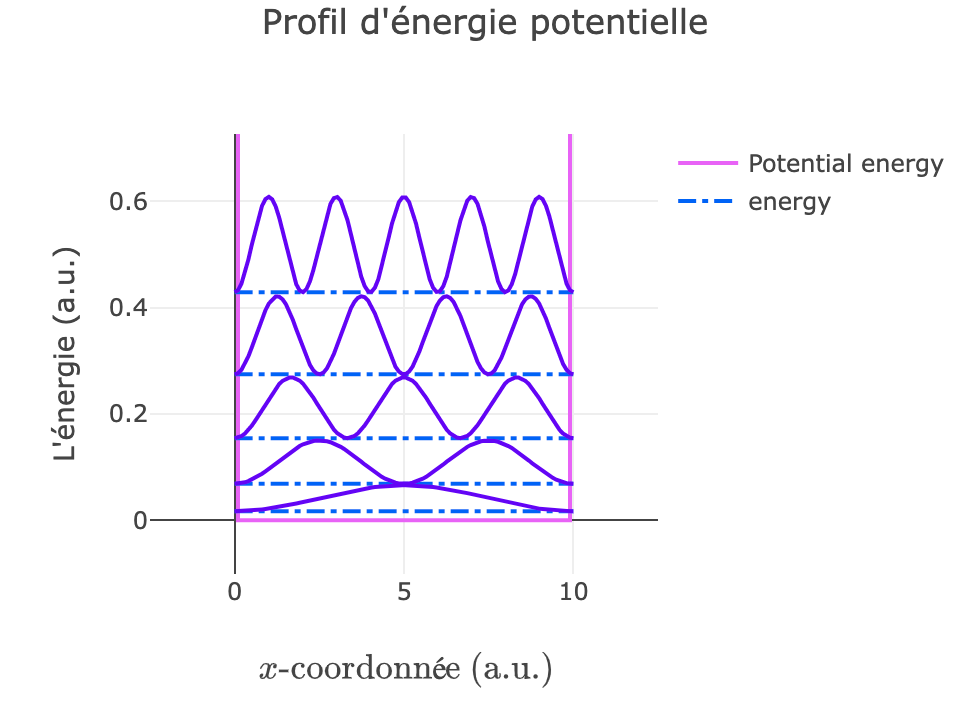
\includegraphics[width=10cm]{PI.png}
    \label{fig:enter-label}
\end{figure}

\begin{breakbox}
\noindent We notice that $\phi_n'$ seems to be discontinuous at the potential discontinuities, i.e., at $x=0$ and $x=a$. It is important to emphasize the boundary conditions and to play with the width and height of the well. For example, increasing the width decreases the energy for a given mode.\\ \\
\textit{General rule: $\phi'$ is continuous at finite potential discontinuities, is often not continuous at infinite discontinuities.}
\end{breakbox}

\medskip

\noindent \textbf{2.c)} Mathematically find the discontinuity of the derivative of $\phi_n$ (compute $\phi_n'(0+)$ and conclude).\\

\begin{breakbox}
    \noindent We have $$\phi_n'(x) = \sqrt{\frac{4mE_n}{a\hbar^2}}\cos\left(\sqrt{\frac{2mE_n}{\hbar^2}}x\right).$$ 
    \noindent Thus,
    $$\boxed{\phi_n'(0^+) = \sqrt{\frac{4mE_n}{a\hbar^2}} \neq \phi_n'(0^-) = 0.}$$    
\end{breakbox}

\medskip

\noindent \textbf{2.d)} Change and switch to "square potential" mode and see what has changed.\\

\begin{figure}[H]
    \centering
    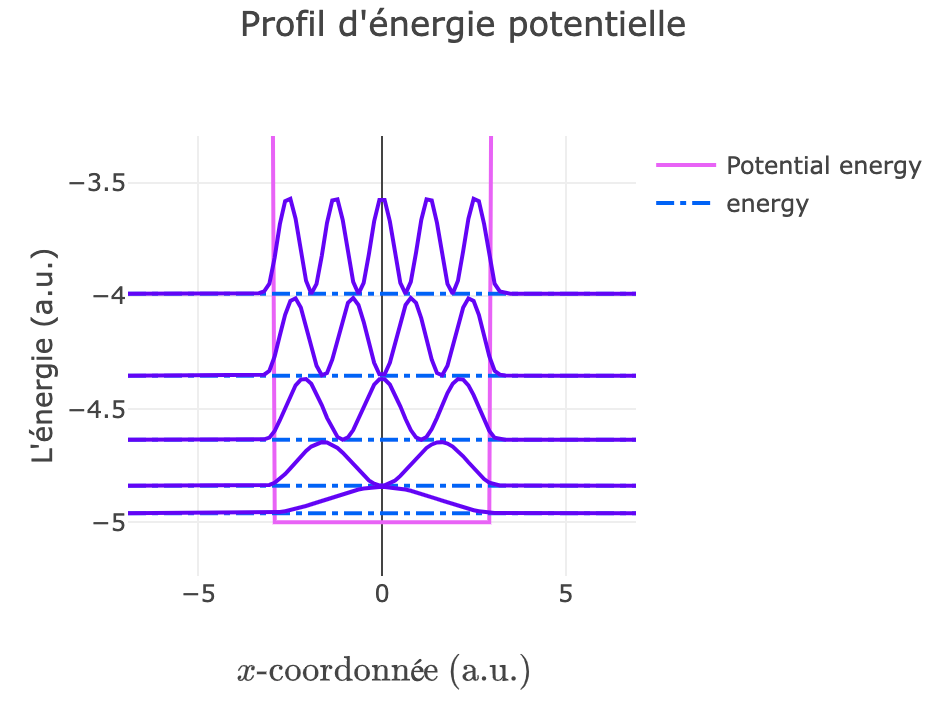
\includegraphics[width=11cm]{PF.png}
    \label{fig:enter-label}
\end{figure}

\begin{figure}[H]
    \centering
    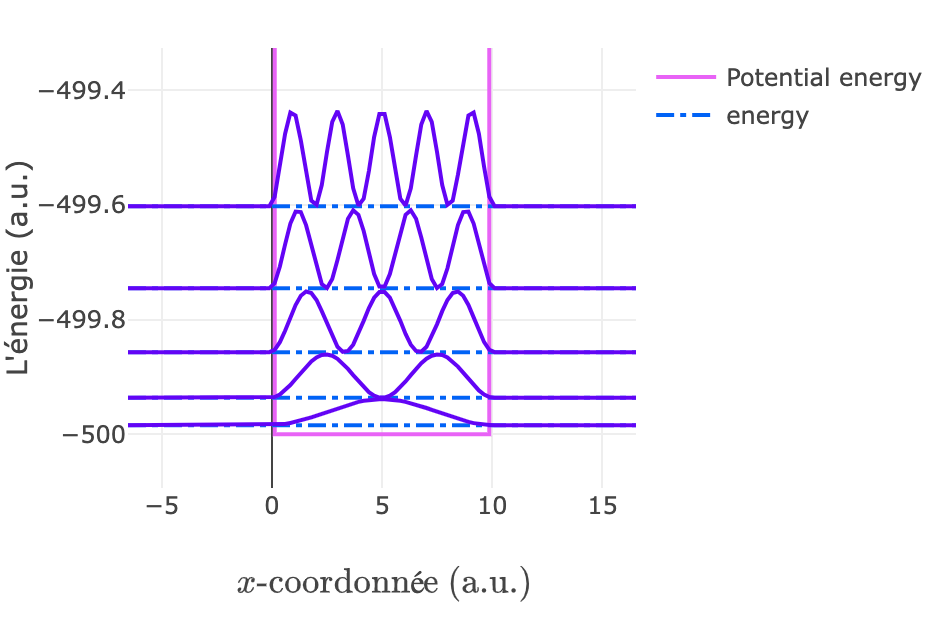
\includegraphics[width=11cm]{PF2.png}
    \label{fig:enter-label}
\end{figure}

\begin{breakbox}
    \noindent We notice that the condition of nullity at the boundaries is no longer respected. To understand concretely the transition, we can start with $V_0 = 500$: then we see that the wave functions are almost the same as in the case of the infinite well. In particular, the wave functions are zero at the boundaries and their derivatives seem to be discontinuous there. \\ \\
    If we now switch to $V_0 = 5$, we notice that the condition of nullity at the boundaries is no longer respected. In fact, inside the well, we still have sinusoidal solutions, but outside the well, we have real decreasing exponentials (make the link with the two types of solutions found in exercise 1 of this tutorial). In this situation, we also see that the derivative at the boundaries of the wave functions is now continuous.    
\end{breakbox}

\medskip

\medskip

\noindent To understand what happens when the well is finite, we consider the part $x>0$. We then consider a particle with energy $E$ coming from $x<a$. It encounters a potential barrier $U_0>E$ at $x=a$.\\

\noindent \textbf{2.e)} Determine the form of the wave functions $\psi(x,t)= \phi(x) e^{-i \frac{Et}{\hbar}}$ for $x>a$.\\

\begin{breakbox}
    \noindent We apply the Schrödinger equation to $\psi(x,t)= \phi(x) e^{-i \frac{Et}{\hbar}}$. For $x>a$, we must take into account the potential $U_0$, so the Schrödinger equation is:
    \begin{equation*}
        i\hbar\frac{\partial\psi(x,t)}{\partial t}= -\frac{\hbar ^2}{2m}\frac{\partial^2\psi(x,t)}{\partial x^2}+U_0\psi(x,t)  
    \end{equation*}

    \noindent By applying the result obtained in the first exercise, we obtain the differential equation for $\phi$:

    \begin{equation*}
        \phi^{''}(x)+\frac{2m(E-U_0)}{\hbar^2}\phi(x)=0.
    \end{equation*}

    \noindent $\displaystyle E-U_0<0$; so, by setting $\displaystyle k_{2}=\frac{2m(U_0-E)}{\hbar^2}$, we obtain a solution of the form :
    $$\phi(x) = Ce^{-k_{2}x} + De^{k_{2}x}.$$

    \noindent Since the solution cannot diverge at +$\infty$, we must have $D=0$, so we obtain the following solution:
    $$\boxed{\phi(x) = Ce^{-k_{2}x} \text{ then } \psi(x,t) = Ce^{k_{2}x}e^{\frac{-iEt}{\hbar}}.}$$

    \noindent The solution is an evanescent wave: it is a wave that does not propagate and decreases.

    \begin{figure}[H]
        \centering
        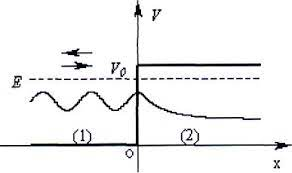
\includegraphics[width = 7cm]{Ondes_evanescentes.jpeg}
        \caption{Evanescent wave}
        \label{fig:enter-label}
    \end{figure}

    \noindent \textit{Remark: In the well for $0<x<a$, the wave function is of the form:}
    
    $$\phi(x) = A \sin(\sqrt{\frac{2mE}{\hbar^2}}x)+B \cos(\sqrt{\frac{2mE}{\hbar^2}}x).$$
    
    \noindent \textit{For $x<0$, by applying the same method as before,}
    
    $$\phi(x) = Fe^{k_{2}x}.$$
    
    \noindent \textit{To determine A, B, C, and F, we use the continuity of $\phi(x)$ and its derivative at $x=0$ and $x=a$ (see Tutorial 2 on tunneling microscope).}
\end{breakbox}

\subsection{Heisenberg's Uncertainty Principle (Bonus)}

\noindent \textbf{3.a)} Recall Heisenberg's uncertainty principle by redefining the two terms involved.\\

\begin{breakbox}
    \noindent Heisenberg's uncertainty principle, or the uncertainty principle, is written as follows:
    \[
        \boxed{\sigma_x\sigma_p \ge \frac{\hbar}{2}.}
    \]
    \noindent We recall that  
    $$\sigma_x^2 = \langle X^2 \rangle_{\psi} - \langle X \rangle_{\psi}^2 \text{ and } \sigma_p^2 = \langle p^2 \rangle_{\psi} - \langle p \rangle_{\psi}^2.$$
    \noindent And in general, for any operator A: 
    $$\boxed{\langle A \rangle_{\psi} = \int \psi^* A \psi \operatorname{dP}.}$$
\end{breakbox}

\medskip

\noindent \textbf{3.b)} Calculate $\langle X \rangle_{\phi_n}$ using the wave functions of the infinite quantum well. \\

\begin{breakbox}
    \noindent We have
    \begin{align*}
        \langle X \rangle_{\phi_n} &= \int_{0}^{a} \phi_n^{*} x \phi_n \mathrm{d}x \\
        &= \int_{0}^{a} \frac{2}{a}x\sin^{2}\left(\sqrt{\frac{2mE_n}{\hbar^2}}x\right) \mathrm{d}x \\
        &= \int_{0}^{a} \frac{2}{a}x\sin^{2}\left(\sqrt{\frac{n\pi}{a}}x\right) \mathrm{d}x \\
        &= \frac{2a}{n^2\pi^2} \int_{0}^{n\pi} X \sin^{2}(X) \mathrm{d}X.
    \end{align*}
    \noindent By making the change of variable $\displaystyle \frac{n\pi}{a}x = X$.\\ \\
    \noindent We calculate separately, using integration by parts (the result can be given to the students):
    \begin{align*}
        \int_{0}^{b} x\sin^{2}(x) \, \mathrm{d}x &= \int_{0}^{b} x\left(\frac{1-\cos(2x)}{2}\right) \, \mathrm{d}x \\
        &= \left[x \frac{x - \frac{\sin(2x)}{2}}{2}\right] - \int_{0}^{b} x - \frac{1}{2}\sin(2x) \, \mathrm{d}x \\
        &= \frac{b^2}{2} -\frac{b}{4}\sin(2b) - \frac{b^2}{4} +\frac{1}{4}\left[-\frac{\cos(2x)}{2}\right

] \\
        &= \frac{b^2 - b\sin(2b) + \frac{1-\cos(2b)}{2}}{4}.
    \end{align*}

    \noindent Finally:
    $$\boxed{\langle X \rangle_{\phi_n} = \frac{2a}{n^2\pi^2}\frac{n^2\pi^2}{4} = \frac{a}{2}.}$$
\end{breakbox}

\medskip

\noindent \textbf{3.c)} Verify on the website that the inequality is satisfied.\\

\begin{breakbox}
    \noindent On the website, go to the "Observables" tab at the bottom of the page, then choose "Heisenberg Uncertainty Principle" from the dropdown menu. We can see that the curve remains above $\displaystyle \frac{\hbar}{2}$.
\end{breakbox}

\medskip

\noindent \textbf{3.d)} Discuss the physical interpretation of this inequality by relating it to its name of uncertainty principle.\\

\begin{breakbox}
    \noindent This inequality shows that there is a theoretical limit to the precision with which two physical properties of the same particle can be simultaneously known. For example, the better the measurement of position, the less precise the measurement of momentum will be, and vice versa.    
\end{breakbox}
\newpage
\section{Thermal diffusion in a cube}

\noindent The purpose of this section is to draw an analogy between the equations encountered with infinite quantum wells (cf. Quantum Physics TD 1 which will soon be addressed) and those of thermal diffusion in a solid with homogeneous boundary conditions (as described below).
In both cases:

\begin{itemize}
    \item Solving so-called "transport" equations;
    \item Observing quantification of solutions, i.e., eigenmodes for temperature propagation in one case or probability of presence in the other.
\end{itemize}

\noindent Consider a solid of infinite height along $\vec{e_y}$ and of width $L$ along $\vec{e_x}$ in a liquid assumed to be infinite at temperature $T_f$, assumed constant and uniform.

\begin{figure}[htbp]
    \centering
    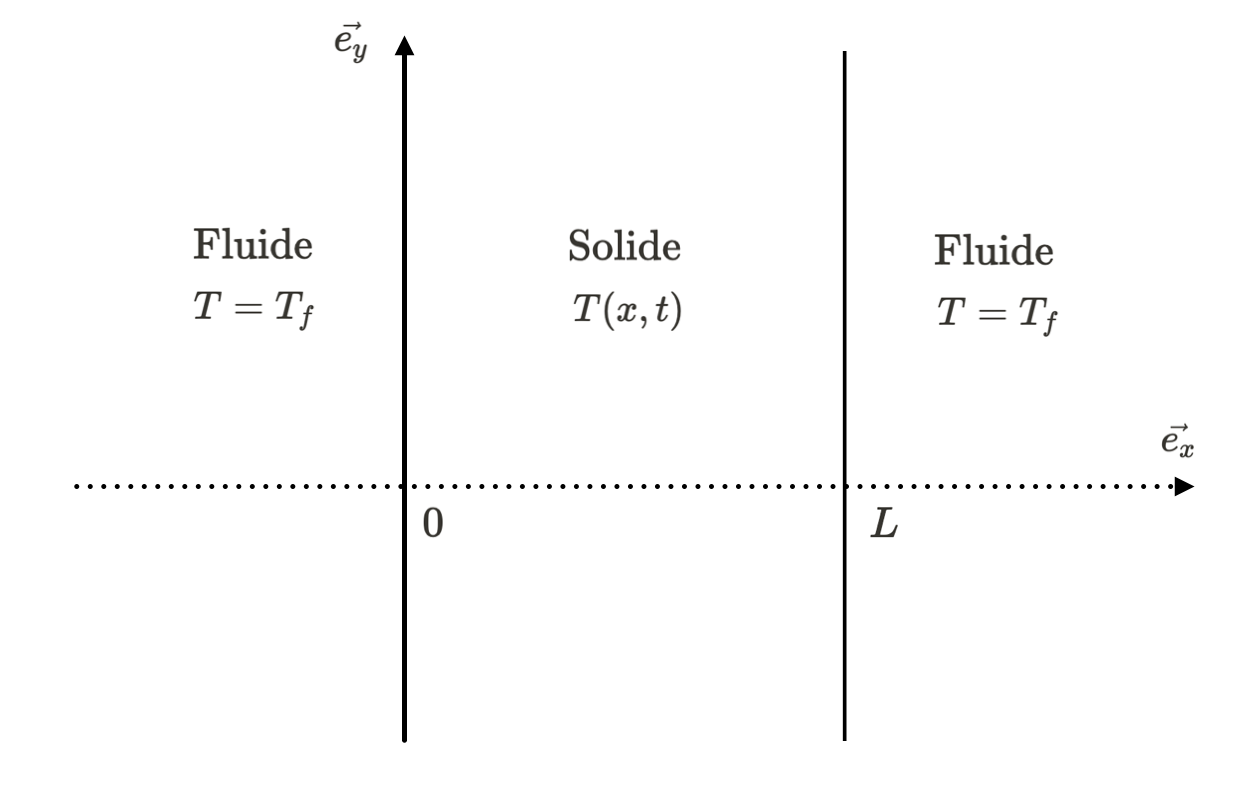
\includegraphics[width=0.5\textwidth]{TD1_2024_EN_Corr_TEX/Scheme_FR.png}
    \caption{Problem scheme}
    \label{fig:schema_diff_thermique}
\end{figure}

\noindent We seek to determine the behavior of the temperature $T(x,t)$ in the solid as a function of position $x$ and time $t$.
The differential equation satisfied by $\theta(x,t) = T(x,t) - T_f$ is \textbf{the heat equation}. It is given by:

\begin{equation}
\frac{\partial \theta}{\partial t} = D \nabla^2 \theta
\label{exocube}
\end{equation}

\noindent where $D = \displaystyle \frac{\lambda}{\rho c_P}$ is the thermal diffusivity of the solid, with $\lambda$ its thermal conductivity, $\rho$ its density, $c_P$ its specific heat capacity at constant pressure.\\ \\
\noindent \textbf{1.a)} By using the method of separation of variables, propose a form of the solution of equation (\ref{exocube}) and write the independent equations of time and space respectively. We will call the introduced constant $\displaystyle -\frac{1}{\tau}$.\\

\begin{breakbox}
    \noindent By separation of variables, $\theta(x,t) = \varphi(x)g(t)$. The equations are therefore as follows for $x \in [0,L]$ and $t > 0$:
    \\
    $$\boxed{
    \begin{cases}
        g'(t) + \frac{1}{\tau}g(t) = 0 \\
        \varphi''(x) + \frac{1}{\tau D}\varphi(x) = 0
    \end{cases},}$$
    \\
    with $\tau \in \mathbb{R}$.
\end{breakbox}

\medskip

\noindent \textbf{1.b)} Provide the boundary conditions satisfied by $\theta(x,t)$.\\

\begin{breakbox}
    \noindent In the fluid, the temperature is assumed constant and uniform, thus:
    $$\boxed{\theta(0,t) = \theta(L, t) = T_f - T_f = 0.}$$
\end{breakbox}

\medskip

\noindent \textbf{2)} Give the general form of the solution of the time-dependent equation. What is the sign of $-\frac{1}{\tau}$? To what is $\tau$ homogeneous?\\

\begin{breakbox}
    \noindent We have: $$\boxed{g(t) = A e^{-\frac{t}{\tau}} \text{ where }A \in \mathbb{R}.}$$ We necessarily have $\displaystyle \frac{1}{\tau} > 0$ for the solution not to diverge.
    $\tau$ is homogeneous to time.
\end{breakbox}

\medskip

\noindent \textbf{3.a)} Give the general form of the solution of the space-dependent equation.\\

\begin{breakbox}
    \noindent $$\boxed{\varphi(x) = C \cos(\sqrt{\frac{1}{\tau D}}x) + E \sin(\sqrt{\frac{1}{\tau D}}x) \text{ where } C, E \in \mathbb{R}.}$$
\end{breakbox}

\medskip

\noindent \textbf{3.b)} Simplify this expression using the boundary condition at $x = 0$.\\

\begin{breakbox}
    \noindent At $x=0$, we have $\varphi(0) = C = 0.$
    Thus, the solution is written as $\boxed{\varphi(x) = E \sin(\sqrt{\frac{1}{\tau D}}x)$ for $x \in \mathbb{R}}$.
\end{breakbox}

\medskip

\noindent \textbf{3.c)} Using the boundary condition imposed at $x=L$, give the allowed values for $\displaystyle \frac{1}{\tau}$.\\

\begin{breakbox}
    \noindent We note the appearance of eigenmodes, i.e., discrete values allowed for the constant $\displaystyle \frac{1}{\tau_n}$.
    Indeed, we have: $$\theta(L,t) = 0 \Rightarrow \sin(\sqrt{\frac{1}{\tau D}}L) = 0 \Rightarrow \sqrt{\frac{1}{\tau D}}L = n\pi \Rightarrow \boxed{\frac{1}{\tau_n} = \frac{D\pi^2}{L^2}n^2, \text{ where } n \in \mathbb{N}.}$$
\end{breakbox}

\medskip

\noindent \textbf{3.d)} What can be said about the general form of $\theta(x,t)$?\\

\begin{breakbox}
    \noindent The eigenmodes of the form $\displaystyle \varphi_n(x) = A_n \sin(\sqrt{\frac{1}{\tau_n D}}x)$ are such that:
    $$\theta_n(x,t) = A_n e^{-\frac{t}{\tau_n}} \sin(\sqrt{\frac{1}{\tau_n D}}x).$$ The general solution is therefore an infinite sum of these eigenmodes:
    $$\boxed{\theta(x,t) = \sum_{n=0}^{\infty} A_n e^{-\frac{t}{\tau_n}} \sin(\sqrt{\frac{1}{\tau_n D}}x) = \sum_{n=0}^{\infty} A_n e^{-\frac{D\pi^2}{L^2}n^2 t} \sin(\frac{n\pi}{L}x).}$$
\end{breakbox}

\medskip

\noindent In the case of a particle in an infinite quantum well of length $L$ with a potential (a case that will be addressed in Quantum Physics TD 1 to be held on Friday, 01/03), as in part \textbf{1.3} we seek the eigenmodes of the Schrödinger equation by separation of variables, to obtain the \underline{general} solutions of this equation that can be written as:
\begin{equation*}
    \psi(x, t) = \sum_{n=1}^{+\infty}\varphi_n(x) f_n(t).
\end{equation*}

\noindent We find that the solutions to the time-independent Schrödinger equation (i.e., the stationary states of the infinite well),
\begin{equation*}
    -\frac{\hbar^2}{2 m} \varphi_n^{''}(x) = E_n \varphi_n(x),
\end{equation*}

\noindent are functions $\displaystyle \varphi_n(x)=A\sin \left(\frac{n \pi x}{L}\right) \text{ with } n \in \mathbb{N}^{*}, \: A \in \mathbb{R}$. \\

\noindent Furthermore, the temporal dependence $f_n(t)$ of the eigenmode $n$ satisfies the equation:
\begin{equation*}
    f_n'(t) = -i\frac{E_n}{\hbar}f_n(t)
\end{equation*}
And is thus of the form $\displaystyle f_n(t) = B e^{-i\frac{E_n}{\hbar}t}, \: B \in \mathbb{R}$.
\noindent The normalization of each eigenmode requires $\displaystyle AB = \sqrt{\frac{2}{L}}$.
\noindent Thus, the general form $\psi(x,t)$ is:
$$\boxed{\psi(t, x) = \sum_{n=1}^{\infty} \sqrt{\frac{2}{L}} e^{-i\frac{E_n t}{\hbar}} \sin \left(\frac{n \pi x}{L}\right)}$$
with 
$
\displaystyle E_n = \frac{n^2 \hbar^2 \pi^2}{2mL^2}, \text{ where } n \in \mathbb{N^*}.
$\\

\noindent \textbf{4.a)} Let's push the analogy a little further. What is the physical significance of $\tau_n$? In the case of the infinite well, what quantity does $\frac{1}{\tau_n}$ compare to?\\

\begin{breakbox}
    \noindent $\tau_n$ is the characteristic time of the exponential decay of temperature in eigenmode $n$. In the case of the infinite quantum well, we identify $\displaystyle \frac{1}{\tau_n}$ with $\displaystyle i\frac{E_n}{\hbar}$.
\end{breakbox}

\medskip

\noindent \textbf{4.b)} How can we define the equivalent of thermal diffusivity $D$ in the case of the infinite quantum well? Can it be given a physical meaning?\\

\begin{breakbox}
    \noindent By expanding we have:
    $$i\frac{E_n}{\hbar} = i\frac{\hbar n^2 \pi^2}{2mL^2} = i\frac{\hbar}{2m} \frac{n^2\pi^2}{L^2}.$$
    By identifying terms in the exponential, we can define a "quantum diffusivity" $\displaystyle D_q = i\frac{\hbar}{2m}$, where $m$ is the mass of the particle.
    This quantity has no physical meaning, but allows to retrieve the expression of the eigenmodes of the infinite quantum well.
\end{breakbox}

\newpage
\section{Exercise VIII: Unsupervised Learning and Clustering}

The main distinction between the k-means and k-means++ algorithms lies in the initialization step. While the k-means algorithm randomly selects the positions of centroids, the k-means++ algorithm employs a more intelligent initialization strategy. The first centroid is chosen randomly from the set of points. Subsequently, each succeeding centroid \(c_{i+1}\) is chosen from the remaining points. The point \(x_j\) is selected with the probability:

\[
\mathbb{P}(x_j = c_{i+1}) = \frac{d(x_j, c_i)^2}{\displaystyle \sum_{k, \text{remaining points}} d(x_k, c_i)^2},
\]

where $d(x_j, c_i)$ represents the distance between centroid \(c_i\) and point \(x_j\). This initialization strategy ensures that points likely to be sufficiently distant from each other.\\ \\
The quality of the solution depends on the initialization. Choosing centroids randomly may lead the algorithm to converge to a good local minimum rather than the global minimum. Additionally, it can reduce the number of iterations required for convergence. This can be particularly useful in cases involving a large number of points, where each step takes a considerable amount of time to compute, and where local minima are more likely to exist.
\newpage
\section{Exercise IX: Probabilistic Classifiers: LDA and QDA}

(a) $\forall k \in \llbracket 1, K \rrbracket,$
\[
    f_k(\mathbf{x}) = \frac{1}{(2\pi)^{d/2}|\Sigma|^{1/2}} \exp(-\frac{1}{2}(\mathbf{x} - \mu_k)^\intercal \Sigma^{-1} (\mathbf{x} - \mu_k)).
\]
Since $t \mapsto \log(t)$ is an increasing function:
\begin{align*}
    \hat{C}(\mathbf{x}) &= \argmax_k f_k(\mathbf{x})\pi_k \\
    &= \argmax_k \log f_k(\mathbf{x})\pi_k \\
    &= \argmax_k \big[- \frac{1}{2} \mathbf{x}^\intercal \Sigma^{-1} \mathbf{x} + \frac{1}{2}\mathbf{x}^\intercal\Sigma^{-1}\mu_k + \frac{1}{2}\mu_k^\intercal\Sigma^{-1}\mathbf{x} - \frac{1}{2}\mu_k^\intercal\Sigma^{-1}\mu_k + \log(\pi_k) + \underbrace{\text{Cst}}_{\substack{\text{does not depend on $k$}}} \big] \\
    &= \argmax_k \big[ \mathbf{x}^\intercal\Sigma^{-1}\mu_k + \mu_k^\intercal\Sigma^{-1}\mathbf{x} - \mu_k^\intercal\Sigma^{-1}\mu_k + 2\log(\pi_k)\big].
\end{align*}
Using the fact that $\mu_k^\intercal\Sigma^{-1}\mathbf{x}$ is a scalar and $\Sigma$ is symmetric (because it is a covariance matrix):
\[
    \mathbf{x}^\intercal\Sigma^{-1}\mu_k = \mu_k^\intercal(\Sigma^{-1})^\intercal \mathbf{x} = \mu_k^\intercal\Sigma^{-1}\mathbf{x}.
\]
Thus,
\[
    \boxed{
    \hat{C}(\mathbf{x}) =\argmax_k \big[ 2\mu_k^\intercal\Sigma^{-1}\mathbf{x} - \mu_k^\intercal\Sigma^{-1}\mu_k + 2\log(\pi_k)\big].
    }
\]
(b) In the case $K=2$, the boundary equation is when $f_1(\mathbf{x}) = f_2(\mathbf{x})$, which gives:
\begin{align*}
   f_1(\mathbf{x}) = f_2(\mathbf{x}) &\iff  2\mu_1^\intercal\Sigma^{-1}\mathbf{x} - \mu_1^\intercal\Sigma^{-1}\mu_1 + 2\log(\pi_1) = 2\mu_2^\intercal\Sigma^{-1}\mathbf{x} - \mu_2^\intercal\Sigma^{-1}\mu_2 + 2\log(\pi_2)\\
   &\iff \boxed{(\mu_1^\intercal - \mu_2^\intercal)\Sigma^{-1}\mathbf{x} = \frac{1}{2}(\mu_1^\intercal\Sigma^{-1}\mu_1 - \mu_2^\intercal\Sigma^{-1}\mu_2) + \log(\frac{\pi_2}{\pi_1}).}
\end{align*}

(c) The MAP rule becomes:
\begin{align*}
    \hat{C}(\mathbf{x}) &= \argmax_k f_k(\mathbf{x})\pi_k \\
    &= \argmax_k \log f_k(\mathbf{x})\pi_k \\
    &= \argmax_k \big[- \frac{1}{2} \mathbf{x}^\intercal \Sigma_k^{-1} \mathbf{x} + \frac{1}{2}\mathbf{x}^\intercal\Sigma_k^{-1}\mu_k + \frac{1}{2}\mu_k^\intercal\Sigma_k^{-1}\mathbf{x} - \frac{1}{2}\mu_k^\intercal\Sigma_k^{-1}\mu_k - \log(\pi_k) - \frac{1}{2}\log|\Sigma_k| \big] \\
    &= \boxed{\argmax_k \big[- \frac{1}{2} \mathbf{x}^\intercal \Sigma_k^{-1} \mathbf{x} + \mu_k^\intercal\Sigma_k^{-1}\mathbf{x} - \frac{1}{2}\mu_k^\intercal\Sigma_k^{-1}\mu_k - \log(\pi_k) - \frac{1}{2}\log|\Sigma_k| \big].}
\end{align*}

(d) QDA stands for "Quadratic Discriminant Analysis." The term "Quadratic" refers to the presence of the term 
\[
- \frac{1}{2} \mathbf{x}^\intercal \Sigma_k^{-1} \mathbf{x}
\]
in the MAP rule. This term is canceled out when $\forall k, \Sigma_k = \Sigma$, but in the case of non-equal covariance assumption, it cannot be eliminated. Therefore, for example, in the scenario of non-equal covariance with $K=2$, the decision boundary equation becomes a quadratic equation, not a linear equation, as seen in question (b).



\newpage

\printbibliography[title={Bibliography}]

\end{document}